\documentclass[11pt,compress,t,notes=noshow]{beamer}
\usepackage[]{graphicx}\usepackage[]{color}
% maxwidth is the original width if it is less than linewidth
% otherwise use linewidth (to make sure the graphics do not exceed the margin)
\makeatletter
\def\maxwidth{ %
  \ifdim\Gin@nat@width>\linewidth
    \linewidth
  \else
    \Gin@nat@width
  \fi
}
\makeatother

\definecolor{fgcolor}{rgb}{0.345, 0.345, 0.345}
\newcommand{\hlnum}[1]{\textcolor[rgb]{0.686,0.059,0.569}{#1}}%
\newcommand{\hlstr}[1]{\textcolor[rgb]{0.192,0.494,0.8}{#1}}%
\newcommand{\hlcom}[1]{\textcolor[rgb]{0.678,0.584,0.686}{\textit{#1}}}%
\newcommand{\hlopt}[1]{\textcolor[rgb]{0,0,0}{#1}}%
\newcommand{\hlstd}[1]{\textcolor[rgb]{0.345,0.345,0.345}{#1}}%
\newcommand{\hlkwa}[1]{\textcolor[rgb]{0.161,0.373,0.58}{\textbf{#1}}}%
\newcommand{\hlkwb}[1]{\textcolor[rgb]{0.69,0.353,0.396}{#1}}%
\newcommand{\hlkwc}[1]{\textcolor[rgb]{0.333,0.667,0.333}{#1}}%
\newcommand{\hlkwd}[1]{\textcolor[rgb]{0.737,0.353,0.396}{\textbf{#1}}}%
\let\hlipl\hlkwb

\usepackage{framed}
\makeatletter
\newenvironment{kframe}{%
 \def\at@end@of@kframe{}%
 \ifinner\ifhmode%
  \def\at@end@of@kframe{\end{minipage}}%
  \begin{minipage}{\columnwidth}%
 \fi\fi%
 \def\FrameCommand##1{\hskip\@totalleftmargin \hskip-\fboxsep
 \colorbox{shadecolor}{##1}\hskip-\fboxsep
     % There is no \\@totalrightmargin, so:
     \hskip-\linewidth \hskip-\@totalleftmargin \hskip\columnwidth}%
 \MakeFramed {\advance\hsize-\width
   \@totalleftmargin\z@ \linewidth\hsize
   \@setminipage}}%
 {\par\unskip\endMakeFramed%
 \at@end@of@kframe}
\makeatother

\definecolor{shadecolor}{rgb}{.97, .97, .97}
\definecolor{messagecolor}{rgb}{0, 0, 0}
\definecolor{warningcolor}{rgb}{1, 0, 1}
\definecolor{errorcolor}{rgb}{1, 0, 0}
\newenvironment{knitrout}{}{} % an empty environment to be redefined in TeX

\usepackage{alltt}
\newcommand{\SweaveOpts}[1]{}  % do not interfere with LaTeX
\newcommand{\SweaveInput}[1]{} % because they are not real TeX commands
\newcommand{\Sexpr}[1]{}       % will only be parsed by R



\usepackage[english]{babel}
\usepackage{dsfont}
\newcommand\bmmax{2}
\usepackage{bm}
\usepackage{bbm}
\usepackage{verbatim}
\usepackage{amsmath}
\usepackage{amsfonts}
\usepackage{csquotes}
\usepackage{multirow}
\usepackage{longtable}
\usepackage{enumerate}
\usepackage[absolute,overlay]{textpos}
\usepackage{psfrag}
\usepackage{algorithm}
\usepackage{algorithmicx}
\usepackage{algpseudocode}
\usepackage{eqnarray}
\usepackage{multimedia}
\usepackage{media9}
\usepackage{arydshln}
\usepackage{tabularx}
\usepackage{placeins}
\usepackage{tikz}
\usepackage{setspace}
\usepackage{wrapfig}
\usepackage{tcolorbox}
\usepackage[export]{adjustbox}
\usepackage{siunitx}
\usetikzlibrary{shapes,arrows,automata,positioning,calc}
\tikzset{
  %Define standard arrow tip
  >=stealth',
  %Define style for boxes
  punkt/.style={
    rectangle,
    rounded corners,
    draw=black, very thick,
    text width=6.5em,
    minimum height=2em,
    text centered},
  % Define arrow style
  pil/.style={
    ->,
    thick,
    shorten <=2pt,
    shorten >=2pt,}
}
\usepackage{subfig}

%new environments

\newenvironment{vbframe}  %frame with breaks and verbatim
{
 \begin{frame}[containsverbatim,allowframebreaks]
}
{
\end{frame}
}

\newenvironment{vframe}  %frame with verbatim without breaks (to avoid numbering one slided frames)
{
 \begin{frame}[containsverbatim]
}
{
\end{frame}
}

\newenvironment{blocki}[1]   % itemize block
{
 \begin{block}{#1}\begin{itemize}
}
{
\end{itemize}\end{block}
}

\newenvironment{fragileframe}[2]{  %fragile frame with framebreaks
\begin{frame}[allowframebreaks, fragile, environment = fragileframe]
\frametitle{#1}
#2}
{\end{frame}}


\newcommand{\myframe}[2]{  %short for frame with framebreaks
\begin{frame}[allowframebreaks]
\frametitle{#1}
#2
\end{frame}}

\newcommand{\remark}[1]{
  \textbf{Remark:} #1
}

%%%%%%%%%%%%%%%%%%%%%%%%%%%%%%%%%%%%%%%%%%%%%%%%%%%%%%%%%%%%%%%%%%%%%%%%%%%%%%%

% basic latex stuff
\newcommand{\pkg}[1]{{\fontseries{b}\selectfont #1}} %fontstyle for R packages
\newcommand{\lz}{\vspace{0.5cm}} %vertical space
\newcommand{\dlz}{\vspace{1cm}} %double vertical space
\newcommand{\oneliner}[1] % Oneliner for important statements
{\begin{block}{}\begin{center}\begin{Large}#1\end{Large}\end{center}\end{block}}


%\usetheme{lmu-lecture}
\usepackage{../style/lmu-lecture}

\let\code=\texttt
\let\proglang=\textsf

\setkeys{Gin}{width=0.9\textwidth}



\title{Deep Learning}
\author{Mina Rezaei}
\institute{Department of Statistics -- LMU Munich}
\date{Winter Semester 2020}

\setbeamertemplate{frametitle}{\expandafter\uppercase\expandafter\insertframetitle}



\begin{document}


\input{../../latex-math/basic-math}

\lecturechapter{8}{Recurrent Neural Networks (RNNs)}
\lecture{Deeplearning}


\begin{frame}
\frametitle{Lecture outline}
\tableofcontents
\end{frame}


%%%%%%%%%%%%%%%%%%%%%%%%%%%%%%%%%%%%%%%%%%%%%%%%%%%%%%%%%%%%%%%%%%
%%%%%%%%%%%%%%%%%%%%%%%%%%%%%%%%%%%%%%%%%%%%%%%%%%%%%%%%%%%%%%%%%%

\begin{frame} {Motivation for RNNs}
  \begin{itemize}
    \item The two major types of neural network architectures that we've seen so far are fully-connected networks and Convolutional Neural Networks (CNNs).
    \item In both cases, the input layers have a fixed size and, therefore, these networks can (typically) only handle fixed-length inputs.
    \item The primary reason for this is that it is not possible to vary the size of the input layer without also varying the number of learnable parameters/weights in the network.
    \item In many cases, we would like to feed \textbf{variable length inputs} to the network.
    \item Common examples of this are \textbf{sequence data} such as time-series, audio and text.
    \item Therefore, we need a new class of neural network architectures that are able to handle such variable length inputs: \textbf{Recurrent Neural Networks (RNNs)}.
  \end{itemize}
\end{frame}


%%%%%%%%%%%%%%%%%%%%%%%%%%%%%%%%%%%%%%%%%%%%%%%%%%%%%%%%%%%%%%%%%%

% \frame{
 
% \frametitle{RNNs - What for?}
%   So far we encountered two types of data: tabular data and image data.
%   Suppose we would like to process sequential inputs, such as
%   \begin{itemize}
%     \item Text data (for text recognition, machine translation, sentiment classification)
%     \item Audio signal analysis (music generation, speech recognition)
%     \item Time series analysis (to predict the stock market,DNA sequence analysis).
%   \end{itemize}
%   Can we do that with a convnet?
%   \begin{itemize}
%     \item[]
%   \end{itemize}
%   \begin{centering}
%   \begin{minipage}{0.42\textwidth}
%     \begin{figure}
%         \only<1-2>{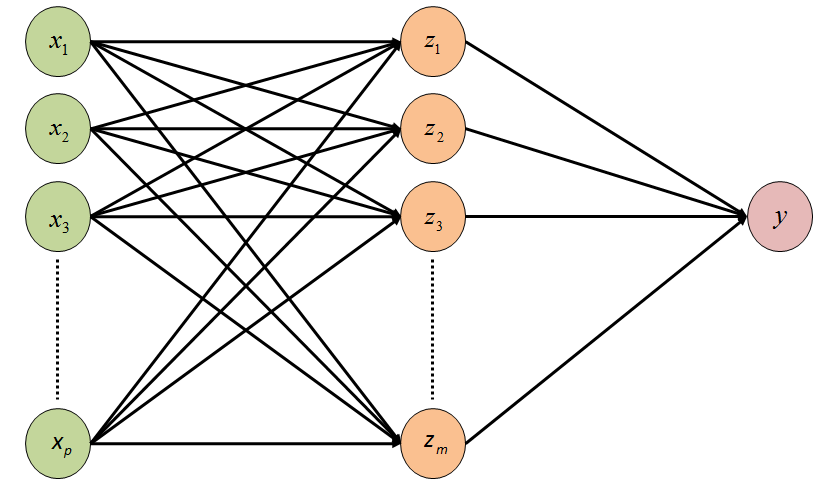
\includegraphics[width=4.5cm]{plots/neuralnet2.png}}
%         \caption{A dense architecture. \textcolor{white}{bla bla bla blabla blabla blabla blabla blabla bla}}
%     \end{figure}
%   \end{minipage}\hfill
%   \begin{minipage}{0.57\textwidth}
%   \vspace{-0.2cm}
%     \begin{itemize}
%       \only<1>{\item[] \textcolor{white}{bla}} % stupid trick to get rid of compiling error
%       \only<2>{\item[] Hardly, the major drawbacks of these models are:} %The major drawbacks of these models for sequential data are:}
%       \only<2>{\begin{itemize}
%         \only<2>{\item \textbf{a fixed input length}. \\ The length of sequential inputs can vary!}
%         \only<2>{\item \textbf{all the examples are independently and identically distributed}. \\ For sequential inputs, there are short and long term temporal dependencies!}
%       \end{itemize}} 
%     \end{itemize}  
%   \end{minipage}
%   \end{centering}
% }
%%%%%%%%%%%%%%%%%%%%%%%%%%%%%%%%%%%%%%%%%%%%%%%%%%%%%%%%%%%%%%%%%%

\section{RNNs -- The basic idea}

\begin{frame} {RNNs - Introduction}
  \begin{itemize}
    \item \small{Suppose we have some text data and our task is to analyse the \textit{sentiment} in the text.
    \item For example, given an input sentence, such as "This is good news.", the network has to classify it as either 'positive' or 'negative'.
    \item We would like to train a simple neural network (such as the one below) to perform the task.}
  \end{itemize}
  \begin{figure}
      \centering
      \scalebox{0.6}{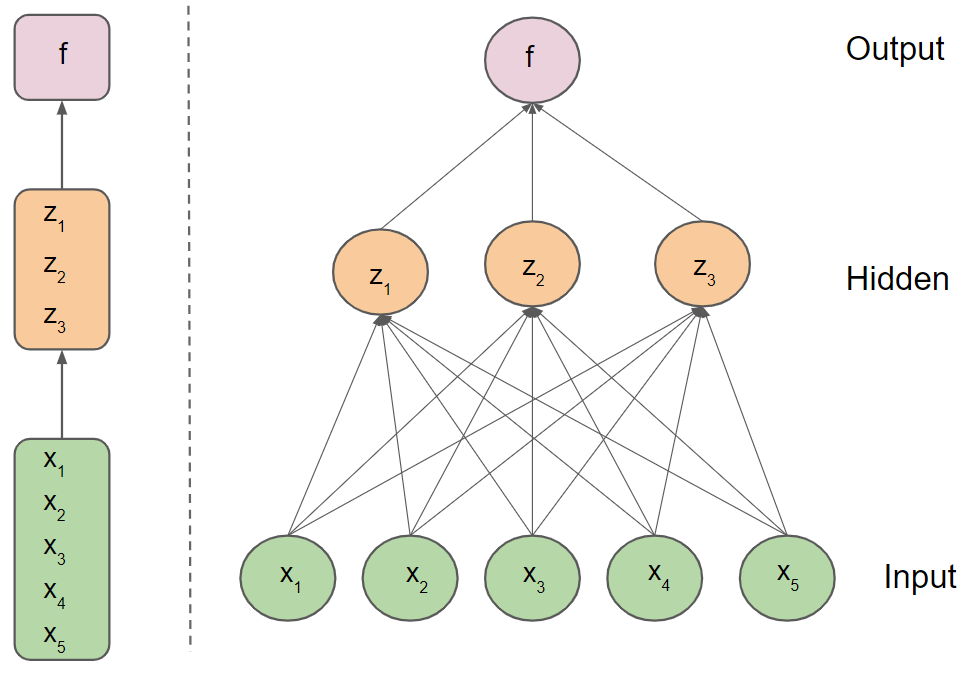
\includegraphics{plots/ffwd.png}}
      \caption{\footnotesize{Two equivalent visualizations of a dense net with a single hidden layer.}}
  \end{figure}
\end{frame}

\begin{frame} {RNNs - Introduction}
  \begin{itemize}
    \item Because sentences can be of varying lengths, we need to modify the dense net architecture to handle such a scenario.
    \item One approach is to draw inspiration from the way a human reads a sentence; that is, one word at a time.
    \item An important cognitive mechanism that makes this possible is "\textbf{short-term memory}".
    \item As we read a sentence from beginning to end, we retain some information about the words that we have already read and use this information to understand the meaning of the entire sentence.
    \item Therefore, in order to feed the words in a sentence sequentially to a neural network, we need to give it the ability to retain some information about past inputs.
    %\item \texbf{We need to track long-term dependencies.}
  \end{itemize}
\end{frame}
 
\begin{frame} {RNNs - Introduction}
  \begin{itemize}
   \item %It's important to note that 
    When words in a sentence are fed to the network one at a time, the inputs are no longer independent. For example, it is much more likely that the word "good" is followed by "morning" rather than "plastic". \textbf{We need to model this (long-term) dependence.} 
    \item %Even though we've decided to feed a single word at a time, 
    Each word must still be encoded as a fixed-length vector because the size of the input layer will remain fixed.
    \item Here, for the sake of the visualization, each word is represented as a 'one-hot coded' vector of length 5. (<eos> = 'end of sequence')
    \begin{figure}
      \centering
      \scalebox{0.55}{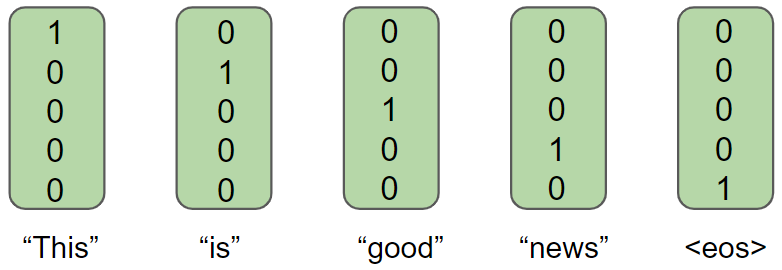
\includegraphics{plots/onehot_1.png}}
  \end{figure}
    (The standard approach is to use word embeddings (more on this later)).
  \end{itemize}
\end{frame}

\begin{frame} {RNNs - Introduction}
  \begin{itemize}
    \item Our goal is to feed the words to the network sequentially in discrete time-steps.
    \item A regular dense neural network with a single hidden layer only has two sets of weights: 'input-to-hidden' weights $\bm{W}$ and 'hidden-to- output' weights $\bm{U}$.
  \end{itemize}
  \begin{figure}
      \centering
      \scalebox{0.7}{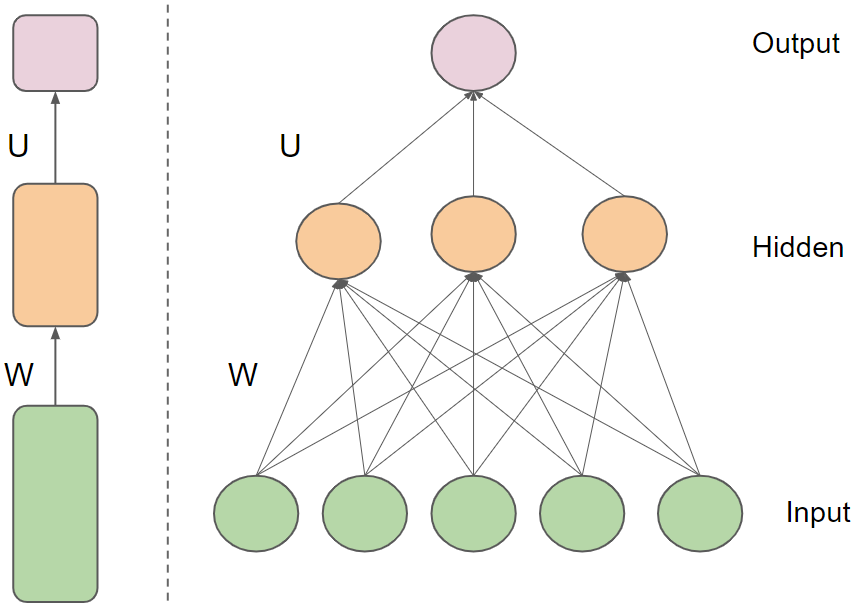
\includegraphics{plots/ffwd1.png}}
  \end{figure}
\end{frame}

\begin{frame} {RNNs - Introduction}
  \begin{itemize}
    \item \small{In order to enable the network to retain information about past inputs, we introduce an \textbf{additional set of weights} $\bm{V}$, from the hidden neurons at time-step $t$ to the hidden neurons at time-step $t+1$.
    \item Having this additional set of weights makes the activations of the hidden layer depend on \textbf{both} the current input and the activations for the \textit{previous} input.}
  \end{itemize}
  \begin{figure}
      \centering
      \scalebox{0.80}{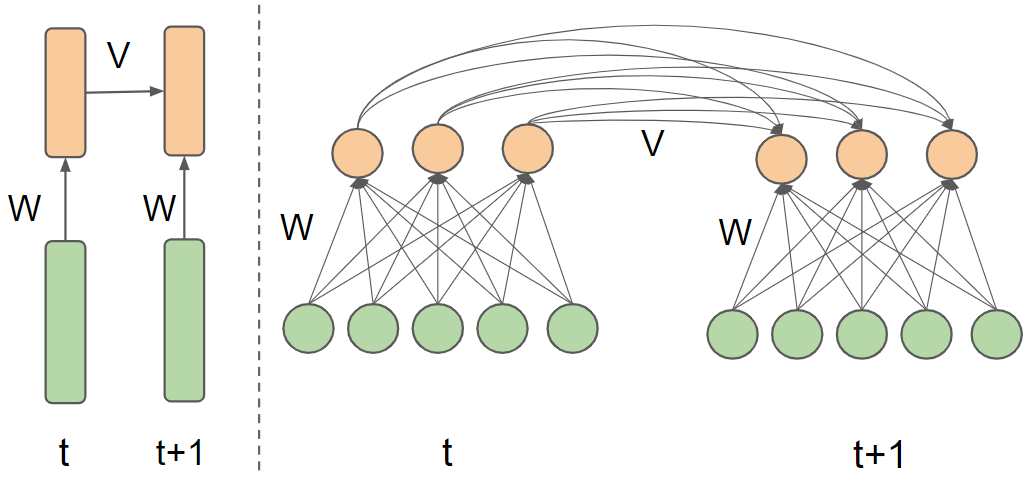
\includegraphics{plots/hidtohid.png}}
      \caption{\footnotesize Input-to-hidden weights $\bm{W}$ and \textbf{hidden-to-hidden} weights $\bm{V}$. The hidden-to-output weights $\bm{U}$ are not shown in the figure.}
  \end{figure}
\end{frame}

\begin{frame} {RNNs - Introduction}
  \begin{itemize}
    \item With this additional set of hidden-to-hidden weights $\bm{V}$, the network is now a Recurrent Neural Network (RNN).
    \item In a regular feed-forward network, the activations of the hidden layer are only computed using the input-hidden weights $\bm{W}$ (and bias $\bm{b}$).
    $$\bm{z}= \sigma(\bm{W}^\top \xv + \bm{b})$$
    \item In an RNN, the activations of the hidden layer (at time-step $t$) are computed using \textit{both} the input-to-hidden weights $W$ and the hidden-to-hidden weights $\bm{V}$.
    $$\bm{z}^{[t]} = \sigma(\mathbf{\textcolor{red}{\bm{V}^\top\bm{z}^{[t-1]}}} + \bm{W}^\top \bm{x}^{[t]} + \bm{b})$$
    \item The vector $\bm{z}^{[t]}$ represents the short-term memory of the RNN because it is a function of the current input $\bm{x}^{[t]}$ and the activations $\bm{z}^{[t-1]}$ of the previous time-step.
    \item Therefore, by recurrence, it contains a "summary" of \textit{all} previous inputs. 
  \end{itemize}
\end{frame}




\begin{frame} {Application example - Sentiment Analysis}
  \begin{itemize}
    \item At $t = 0$, we feed the word "This" to the network and obtain $\bm{z}^{[0]}$.
    \item $\bm{z}^{[0]} = \sigma(\bm{W}^\top \bm{x}^{[0]} + \bm{b})$
  \end{itemize}
  \begin{figure}
      \centering
      \scalebox{0.55}{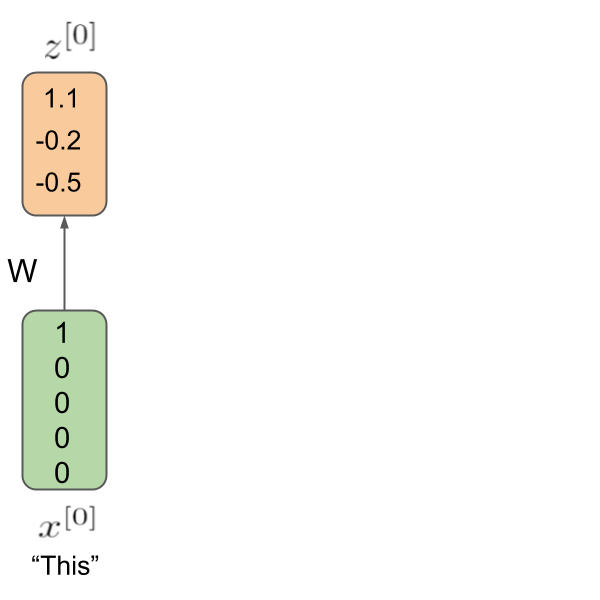
\includegraphics{plots/mto_1.png}}
  \end{figure}
  Because this is the very first input, there is no past state (or, equivalently, the state is initialized to 0).
\end{frame}

\begin{frame} {Application example - Sentiment Analysis}
  \begin{itemize}
    \item At $t = 1$, we feed the second word to the network to obtain $\bm{z}^{[1]}$.
    \item $\bm{z}^{[1]} = \sigma(\bm{V}^\top\textcolor{red}{\bm{z}^{[0]}} + \bm{W}^\top \xv^{[1]} + \bm{b})$
  \end{itemize}
  \begin{figure}
      \centering
      \scalebox{0.55}{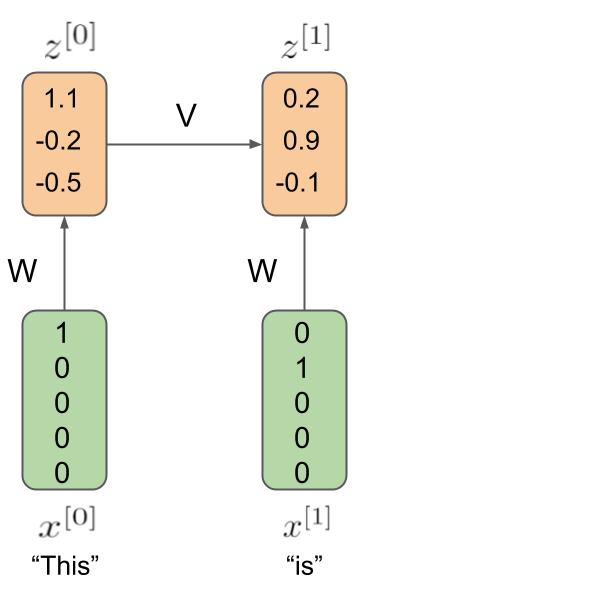
\includegraphics{plots/mto_2.png}}
  \end{figure}
\end{frame}

\begin{frame} {Application example - Sentiment Analysis}
  \begin{itemize}
    \item At $t = 2$, we feed the next word in the sentence.
    \item $\bm{z}^{[2]} = \sigma(\bm{V}^\top\textcolor{red}{\bm{z}^{[1]}} + \bm{W}^\top \xv^{[2]} + \bm{b})$
  \end{itemize}
  \begin{figure}
      \centering
      \scalebox{0.55}{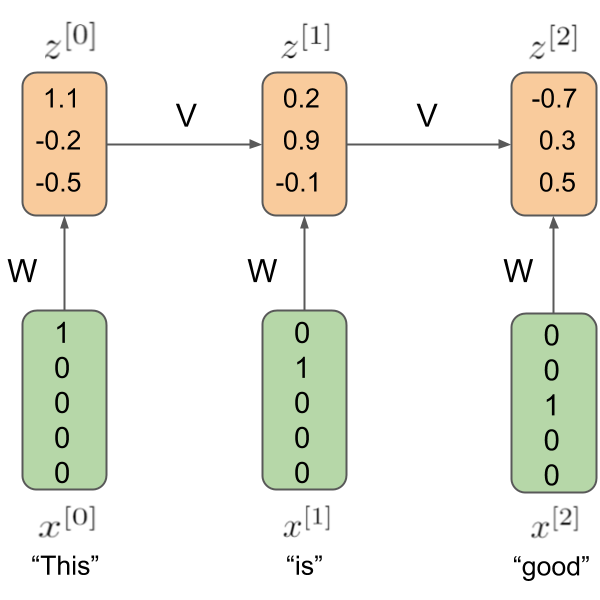
\includegraphics{plots/mto_3.png}}
  \end{figure}
\end{frame}

\begin{frame} {Application example - Sentiment Analysis}
  \begin{itemize}
    \item At $t = 3$, we feed the next word ("news") in the sentence.
    \item $\bm{z}^{[3]} = \sigma(\bm{V}^\top\textcolor{red}{\bm{z}^{[2]}} + \bm{W}^\top \xv^{[3]} + \bm{b})$
  \end{itemize}
  \begin{figure}
      \centering
      \scalebox{0.65}{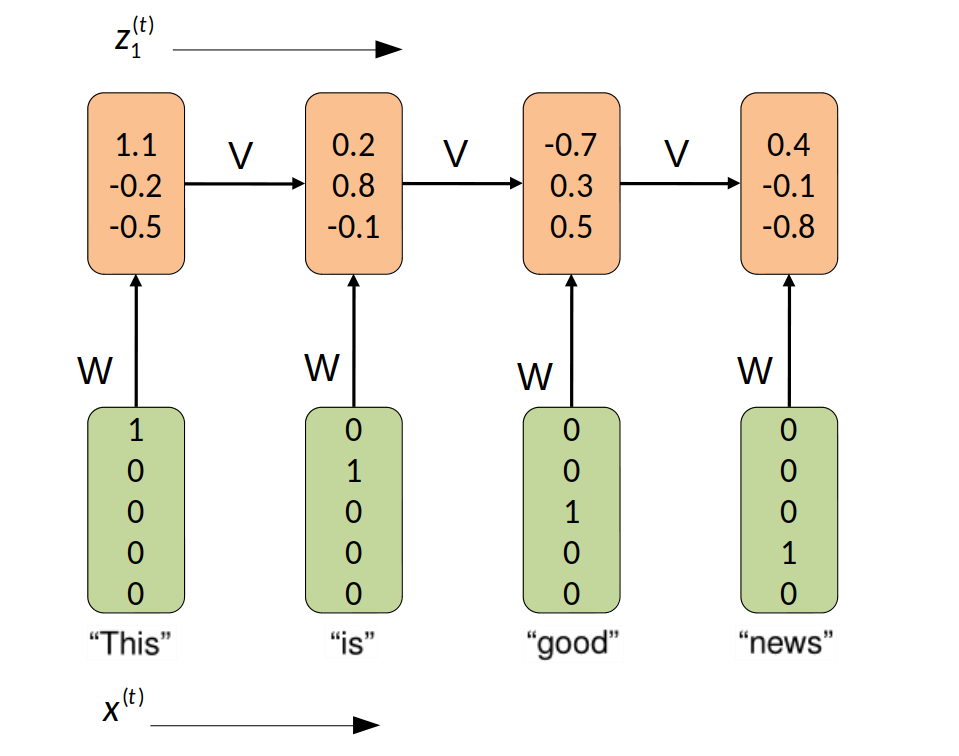
\includegraphics{plots/mto_4.png}}
  \end{figure}
\end{frame}

\begin{frame} {Application example - Sentiment Analysis}
  \begin{itemize}
    \item Once the entire input sequence has been processed, the prediction of the network can be generated by feeding the activations of the final time-step to the output neuron(s).
    \item $f = \sigma (\bm{U}^\top \bm{z}^{[4]} + {c})$, where $c$ is the bias of the output neuron.
  \end{itemize}
  \begin{figure}
      \centering
      \scalebox{0.65}{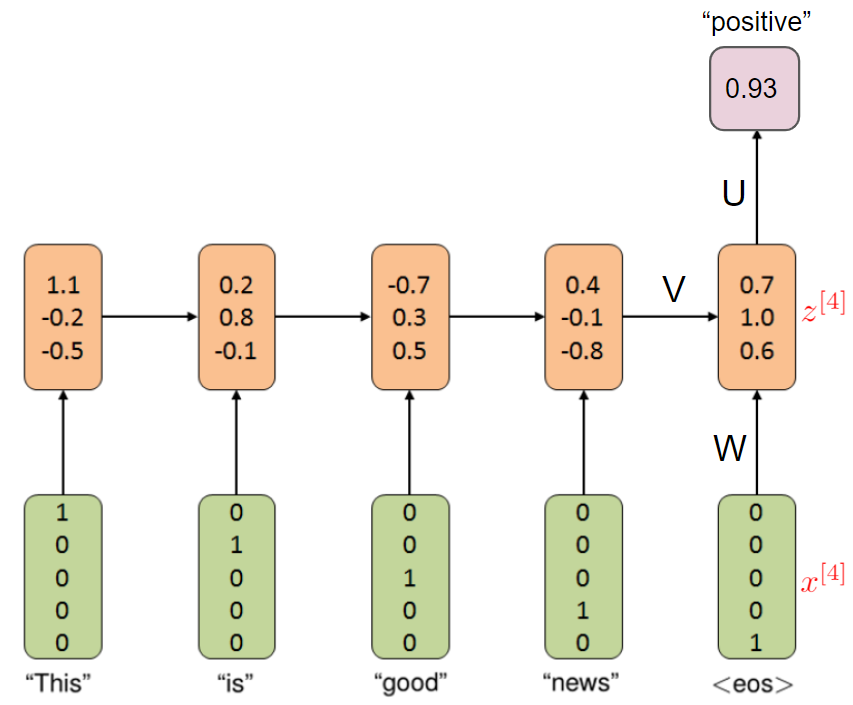
\includegraphics{plots/mto_5.png}}
  \end{figure}
\end{frame}

\begin{frame} {Parameter Sharing}
  \begin{itemize}
    \item This way, the network can process the sentence one word at a time and the length of the network can vary based on the length of the sequence.
    \item It is important to note that no matter how long the input sequence is, the matrices $\bm{W}$ and $\bm{V}$ are the same in every time-step. This is another example of \textbf{parameter sharing}.
    \item Therefore, the number of weights in the network is independent of the length of the input sequence.
  \end{itemize}
\end{frame}

\begin{frame} {Sequence Modeling: -- Design Criteria}

To model sequence we need to:


  \begin{itemize}
    \item Handle variable-length sequence,
    \item Track long-term dependencies,
    \item Maintain information about order,
    \item Share parameter across the sequence.
  \end{itemize}

  \begin{figure}
      \centering
      \scalebox{0.2}{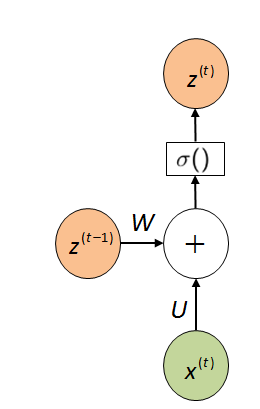
\includegraphics{plots/vanilla_rnn.png}}
      \caption{\footnotesize {Vanilla RNN}}
  \end{figure}

\end{frame}

\begin{frame} {RNNs - Use Case specific architectures}

  \small{RNNs are very versatile. They can be applied to a wide range of tasks.
  
  \begin{figure}
      \centering
      \scalebox{0.9}{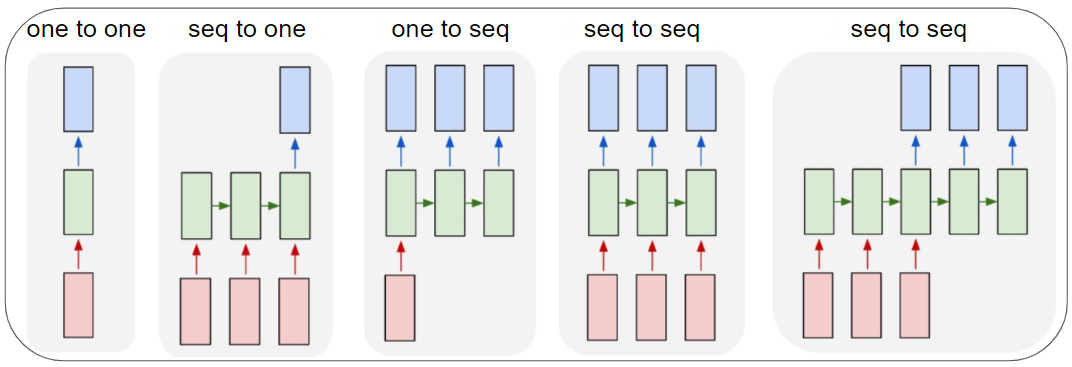
\includegraphics{plots/usecase_1.png}}
      \tiny{\\Credit: Andrej Karpathy}
      \caption{\footnotesize {RNNs can be used in tasks that involve multiple inputs and/or multiple outputs. }}
  \end{figure}
  Examples:}
  \begin{itemize}
    \item \small{Sequence-to-One: Sentiment analysis, document classification.
    \item One-to-Sequence: Image captioning.
    \item Sequence-to-Sequence: Language modelling, machine translation, time-series prediction.}
  \end{itemize}
\end{frame}


%%%%%%%%%%%%%%%%%%%%%%%%%%%%%%%%%%%%%%%%%%%%%%%%%%%%%%%%%%%%%%%%%%
%%%%%%%%%%%%%%%%%%%%%%%%%%%%%%%%%%%%%%%%%%%%%%%%%%%%%%%%%%%%%%%%%%

\section{RNNs - Computational Graph}

\frame{
\frametitle{RNNs - Computational Graph}
  \center
  \begin{figure}%
    \only<1>{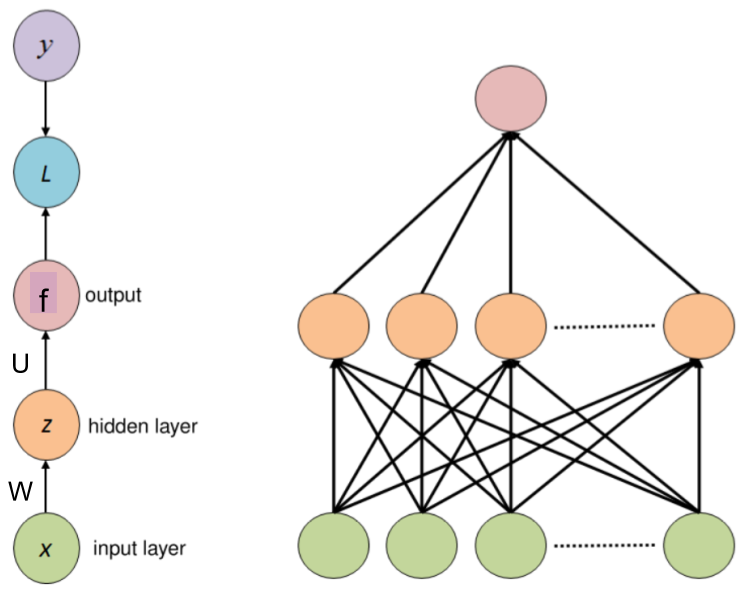
\includegraphics[width=7cm]{plots/rnn_comp1.png}}%
%   \only<2-3>{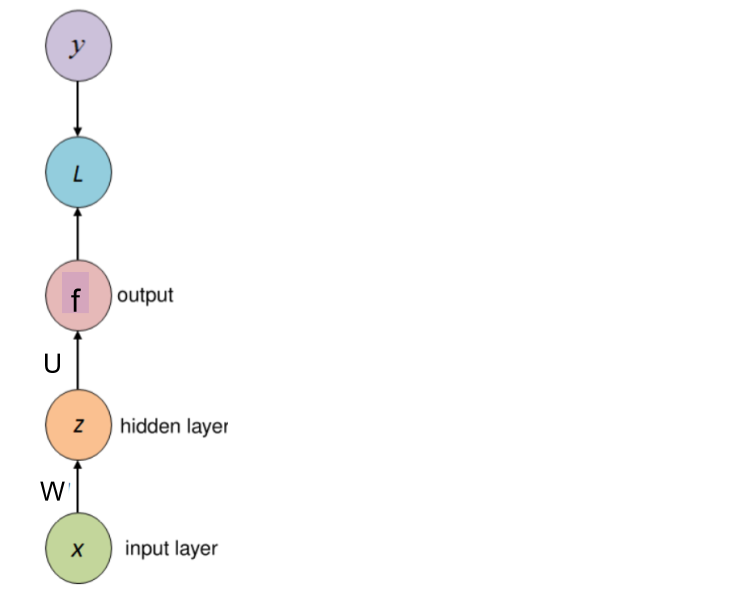
\includegraphics[width=7cm]{plots/rnn_comp2.png}}%
    \only<2>{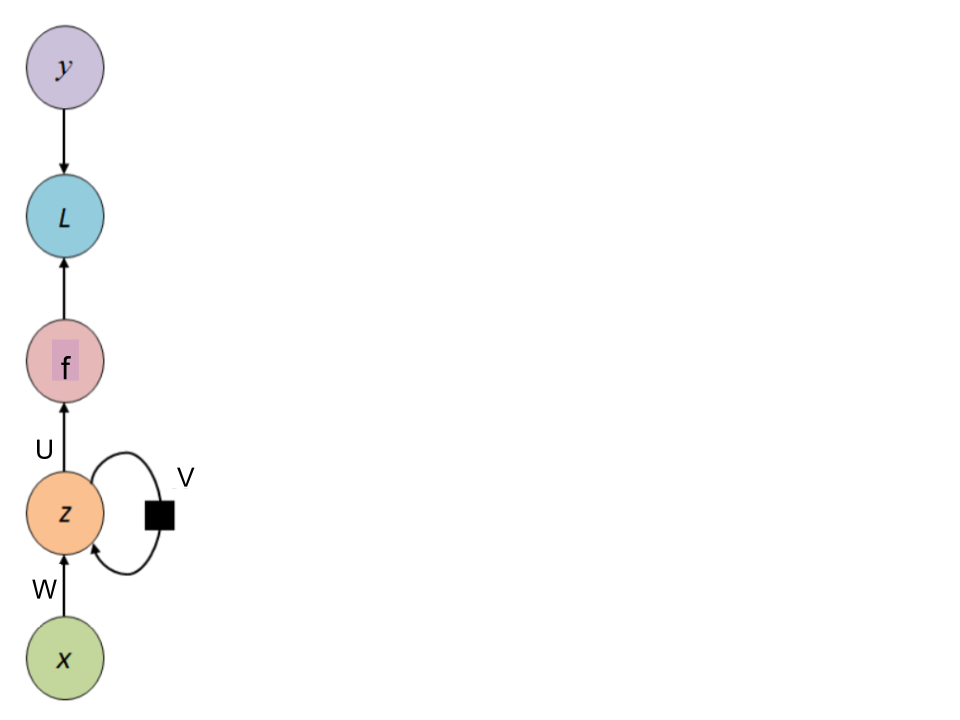
\includegraphics[width=7cm]{plots/rnn_comp3.png}}%
    \only<3-4>{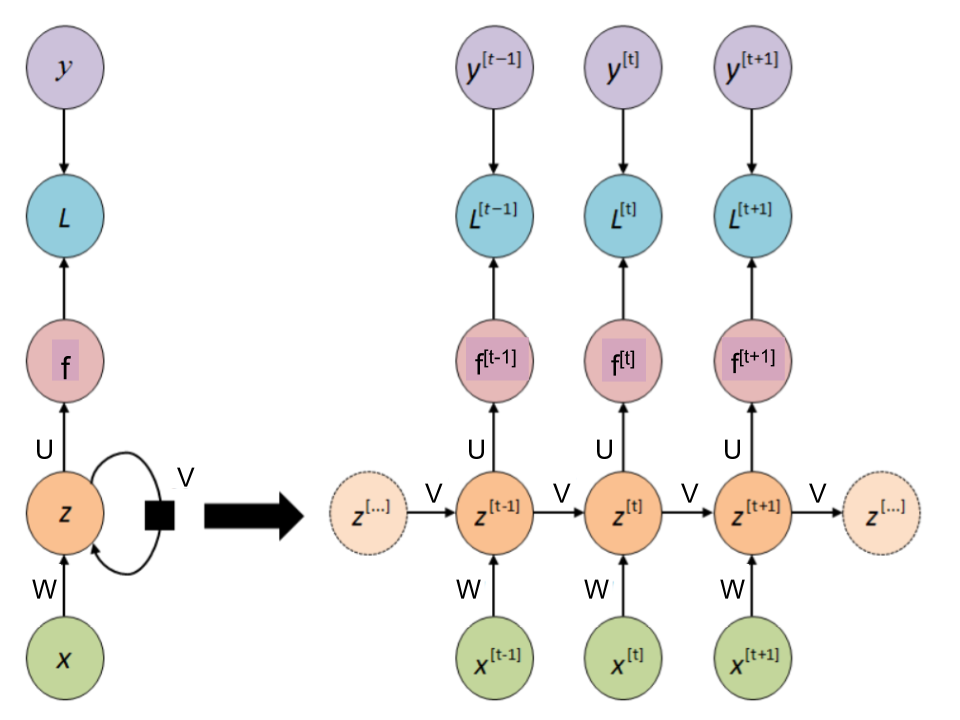
\includegraphics[width=7cm]{plots/rnn_comp8.png}}%
    \only<5>{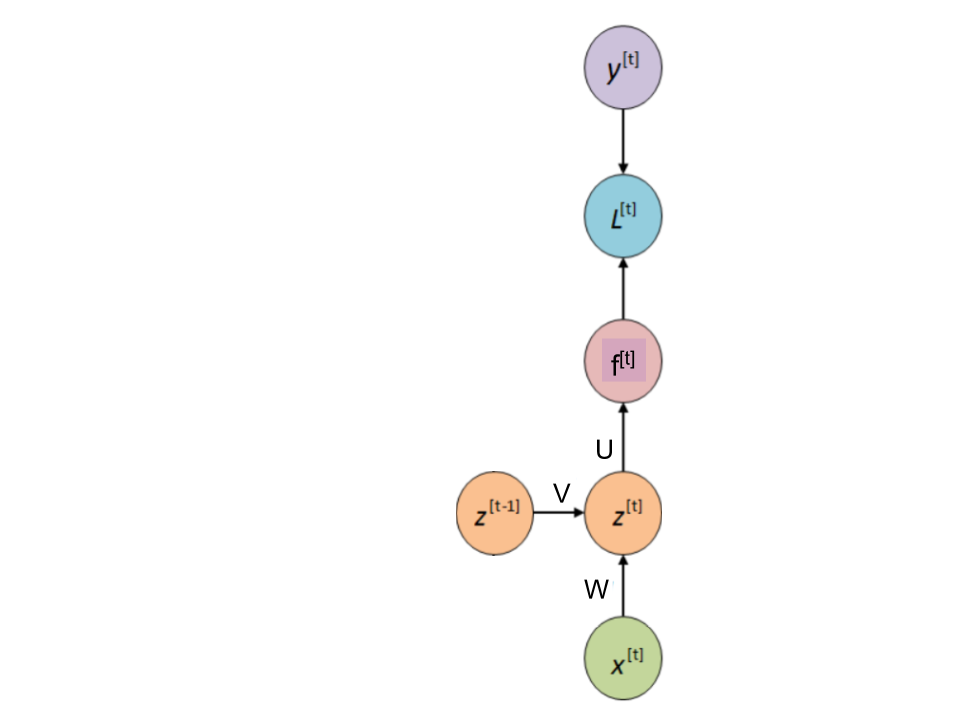
\includegraphics[width=7cm]{plots/rnn_comp5.png}}%
  \end{figure}%
  \vspace{-0.2cm}
  \begin{itemize}
    \only<1>{\item On the left is the computational graph for the dense net on the right. A loss function $L$ measures how far each output
    $f$ is from the corresponding training target $y$. }
    % \only<2-3>{\item In order to derive RNNs we have to extend our notation.}
    % \only<3>{\begin{itemize}
    %   \only<3>{\item So far, we mapped some inputs $x$ to outputs $f$:}
    %   \only<3>{\item[] $f = \tau(c + U^T z) = \tau(c + U^T \sigma(b + W^T x))$}
    %   \only<3>{\item[] ..with $W$ and $U$ being weight matrices.}
    % \end{itemize}}
    \only<2>{\item A helpful way to think of an RNN is as multiple copies of the same network, each passing a message to a successor.}
    \only<2>{\item RNNs are networks with loops, allowing information to persist.}
    \only<3>{\item Things might become more clear if we unfold the architecture.}
    \only<3>{\item We call $\bm{z}^{[t]}$ the \textit{state} of the system at time $t$.}
    \only<3>{\item Recall, the state contains information about the whole past sequence.}
    \only<4>{\item We went from 
      \begin{eqnarray*} 
        f &=& \tau(c + \bm{U}^\top \sigma(\bm{b} + \bm{W}^\top \bm{x})) \text{ for the dense net, to } \\
        f^{[t]} &=& \tau(c + \bm{U}^\top \sigma(\bm{b} + \bm{V}^\top \bm{z}^{[t-1]} + \bm{W}^\top \xv^{[t]})) \text{ for the RNN. }
      \end{eqnarray*}}
    \only<5>{\item Potential computational graph for time-step $t$:}
    \only<5>{\item[] $$f^{[t]} = \tau(c + \bm{U}^\top \sigma(\bm{b} + \bm{V}^\top \bm{z}^{[t-1]} + \bm{W}^\top \xv^{[t]})) $$ }
  \end{itemize}
}


\frame{
\frametitle{RNNs - Computational Graph with recurrent output-hidden connections}

Recurrent connections do not need to map from hidden to hidden neurons!

\center
\begin{figure}
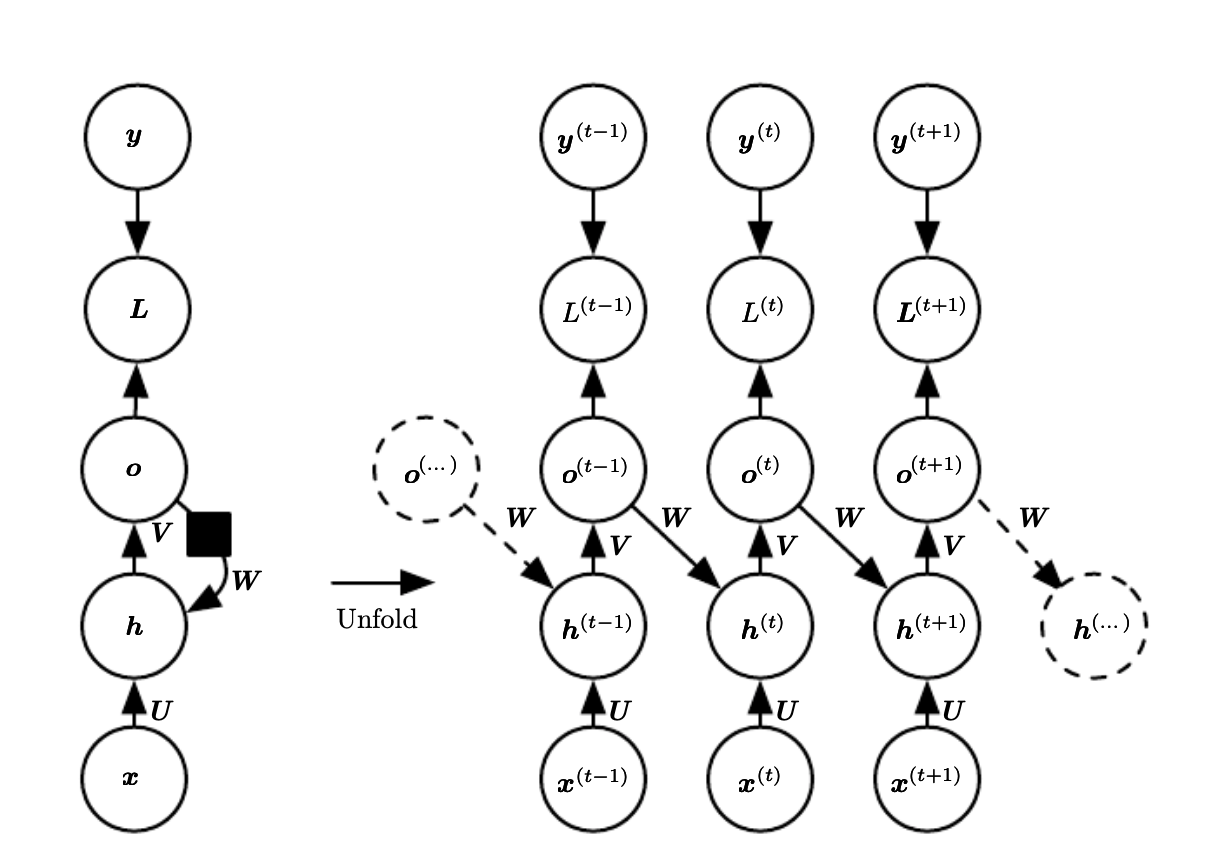
\includegraphics[width=7cm]{plots/rnn_cg_104.png} 
     \tiny{\\ An RNN whose only recurrence is the feedback connection from the output to the hidden layer. At each time stept, the input is $x_t$, the hidden layer activations are $h^{(t)}$, the outputs are $o^{(t)}$, the targets are $y^{(t)}$, and the loss is $L^{(t)}$. (Left) Circuitdiagram. (Right) Unfolded computational graph. The RNN in this figure is trained to put a specific output value into $o$, and $o$ is the only information it is allowed to send to the future. There are no direct connections from $h$ going forward. The previous $h$ is connected to the present only indirectly, via the predictions it was used to produce.}
\end{figure}


}

\frame{
\frametitle{RNNs - Computational Graph for seq to one mapping}

RNNs do not need to produce an output at each time step. Often only one output is produced after processing the whole sequence. 

\center
\begin{figure}
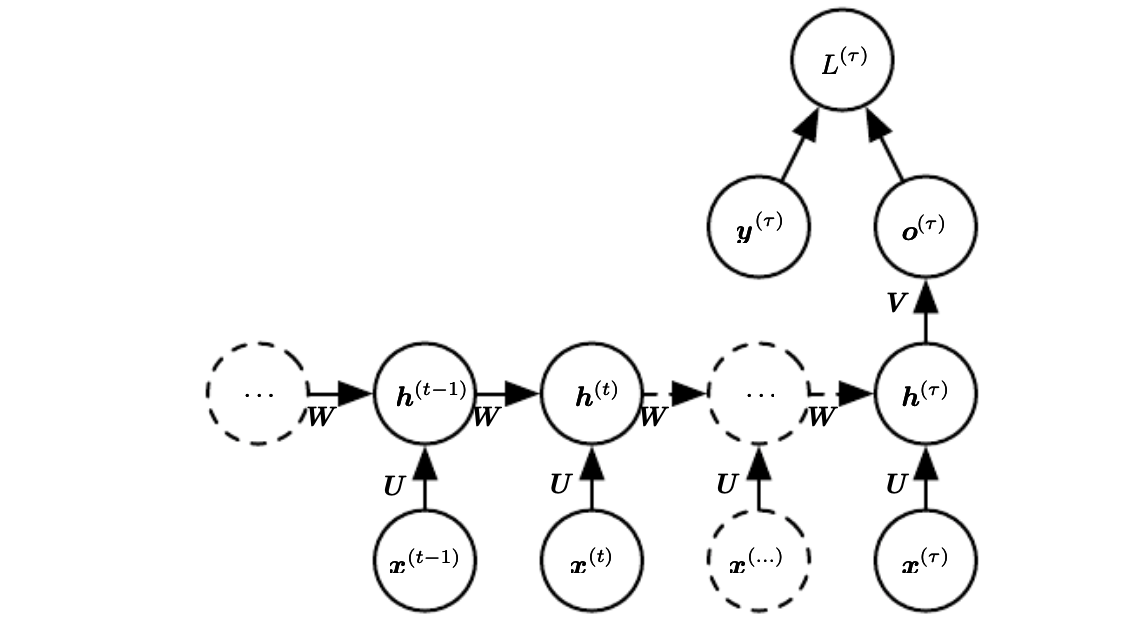
\includegraphics[width=7cm]{plots/rnn_cg_105.png} 
     \tiny{\\Time-unfolded recurrent neural network with a single output at the end of the sequence. Such a network can be used to summarize a sequence and produce a fixed size representation used as input for further processing. There might be a target right at the end (as depicted here), or the gradient on the output $o^{(t)}$ can be obtained by backpropagating from further downstream modules.}
\end{figure}

}



%%%%%%%%%%%%%%%%%%%%%%%%%%%%%%%%%%%%%%%%%%%%%%%%%%%%%%%%%%%%%%%%%%
%%%%%%%%%%%%%%%%%%%%%%%%%%%%%%%%%%%%%%%%%%%%%%%%%%%%%%%%%%%%%%%%%%
\section{Computing the Loss Gradient in RNNs}

\frame{

\frametitle{Backpropagation through time}

  \center
  %\only<1>{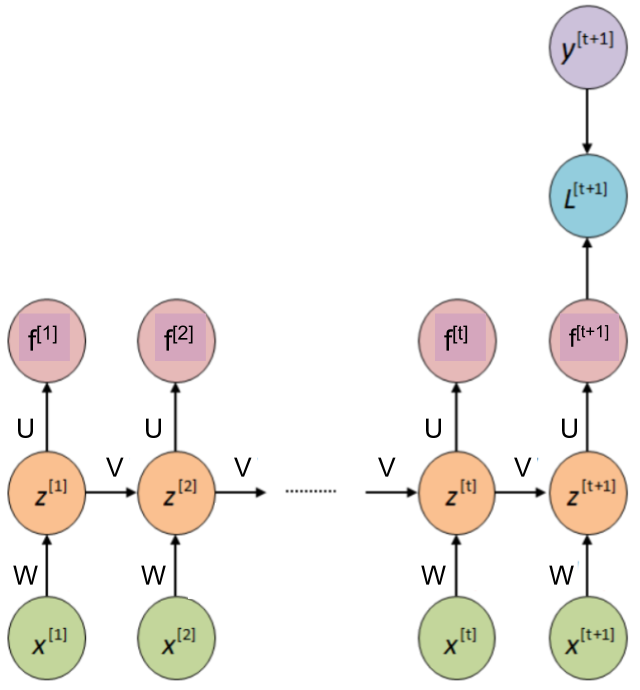
\includegraphics[width=4cm]{plots/rnn_bppt1.png}}%
  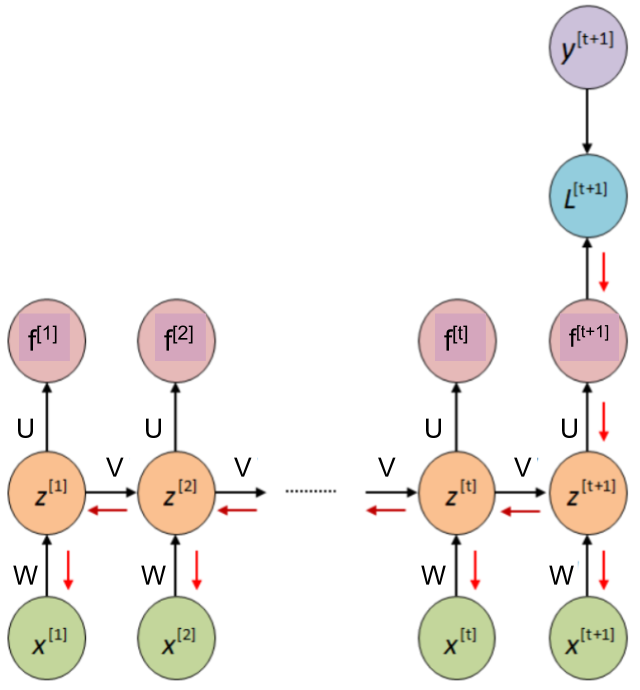
\includegraphics[width=4cm]{plots/rnn_bppt3.png}%

  \begin{itemize}

    \item For training the RNN we need to compute $\frac{d L}{d u_{i,j}}$, $\frac{d L}{d v_{i,j}}$, and $\frac{d L}{d w_{i,j}}$.
    \item To do so, during backpropagation at time step $t$ %for an arbitrary RNN, 
    we may need to compute
    % \item $$\textcolor{white}{\frac{d L}{d z^{[1]}}} = \frac{d L}{d z^{[t]}} \frac{z^{[t]}}{d z^{[t-1]}} \dots \frac{d z^{[2]}}{d z^[1]}$$
    %\only<2>{\item[] $$\frac{d L}{d z^i} = \frac{d L}{d z^{t}} \frac{z^{t}}{d z^{t-1}} \dots \frac{d z^2}{d z^1}$$}
    $$\frac{d L}{d \bm{z}^{[1]}} = \frac{d L}{d \bm{z}^{[t]}} \frac{d \bm{z}^{[t]}}{d \bm{z}^{[t-1]}} \dots \frac{d \bm{z}^{[2]}}{d \bm{z}^{[1]}}$$

  \end{itemize}

}


%%%%%%%%%%%%%%%%%%%%%%%%%%%%%%%%%%%%%%%%%%%%%%%%%%%%%%%%%%%%%%%%%%
%%%%%%%%%%%%%%%%%%%%%%%%%%%%%%%%%%%%%%%%%%%%%%%%%%%%%%%%%%%%%%%%%%
% \begin{vbframe}{Nlp - Example}
%       Example: 
%   \begin{itemize}
%     \item Suppose we only had a vocabulary of four possible letters: \enquote{h}, \enquote{e}, \enquote{l} and \enquote{o}
%     \item We want to train an RNN on the training sequence \enquote{hello}.
%     \item This training sequence is in fact a source of 4 separate training examples:
%       \begin{itemize}
%         \item The probability of \enquote{e} should be likely given the context of \enquote{h}
%         \item \enquote{l} should be likely in the context of \enquote{he}
%         \item \enquote{l} should also be likely given the context of \enquote{hel}
%         \item and \enquote{o} should be likely given the context of \enquote{hell}
%       \end{itemize}
%   \end{itemize}
% \end{vbframe}
%%%%%%%%%%%%%%%%%%%%%%%%%%%%%%%%%%%%%%%%%%%%%%%%%%%%%%%%%%%%%%%%%%
%%%%%%%%%%%%%%%%%%%%%%%%%%%%%%%%%%%%%%%%%%%%%%%%%%%%%%%%%%%%%%%%%%
% \frame{
% 
% \frametitle{Nlp - Example}
% 
% The RNN has a 4-dimensional input and output. The exemplary hidden layer consists of 3 neurons. This diagram shows the activations in the forward pass when the RNN is fed the characters \enquote{hell} as input. The output contains confidences the RNN assigns for the next character.
%   \begin{itemize}
%     \item[]
%   \end{itemize}
%   \begin{minipage}{0.55\textwidth}
%     \begin{figure}
%         \only<1>{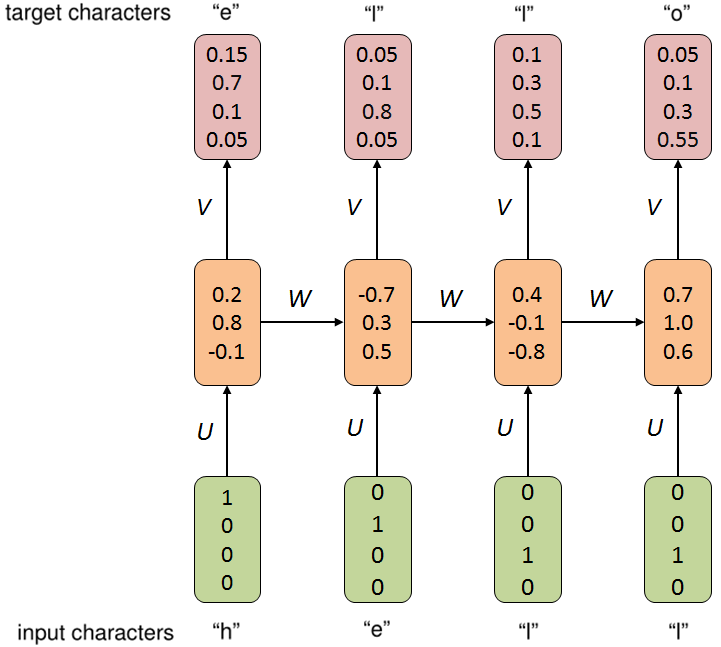
\includegraphics[width=5.5cm]{plots/nlp1.png}}%
%         \only<2>{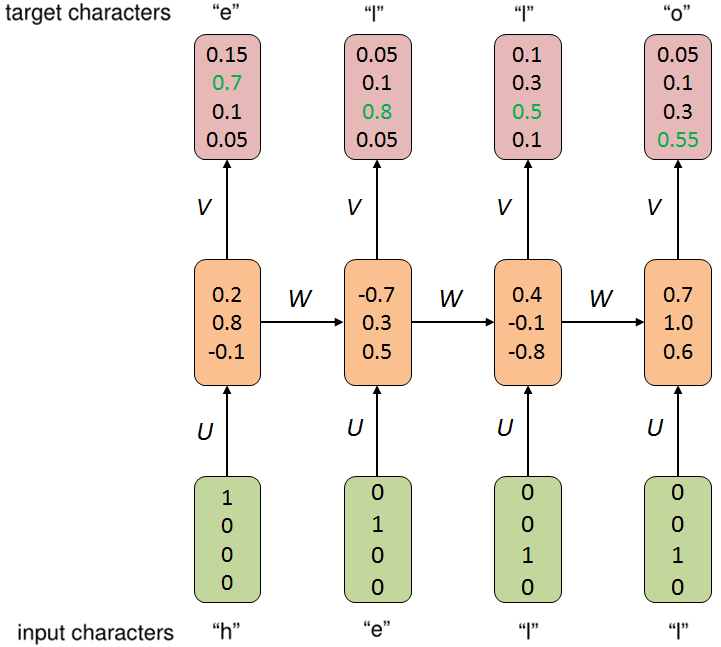
\includegraphics[width=5.5cm]{plots/nlp2.png}}%
%     \end{figure}
%   \end{minipage}%\hfill
%   \begin{minipage}{0.45\textwidth}
%   %\vspace{-0.3cm}
%   
%     \begin{itemize}
%       \only<1>{\item[] \textcolor{white}{Our goal is to increase the confidence for the correct letters (green digits) and decrease the confidence of all others (we could also use a softmax activation to squash the digits to probabilities $\in [0,1]$).}} 
%       \only<2>{\item[] Our goal is to increase the confidence for the correct letters (green digits) and decrease the confidence of all others (we could also use a softmax activation to squash the digits to probabilities $\in [0,1]$).} 
%     \end{itemize}
%   \end{minipage}
%   
% }
%%%%%%%%%%%%%%%%%%%%%%%%%%%%%%%%%%%%%%%%%%%%%%%%%%%%%%%%%%%%%%%%%%
%%%%%%%%%%%%%%%%%%%%%%%%%%%%%%%%%%%%%%%%%%%%%%%%%%%%%%%%%%%%%%%%%%
% \begin{vbframe}{Word Embeddings (Word2vec)}
%   \begin{minipage}{0.4\textwidth}
%     \begin{itemize}
%       \item Data Sparsity: 
%       \item[]
%       $$\text{man} \to \begin{bmatrix}
%                                   0\\
%                                   \vdots\\
%                                   0\\
%                                   1\\
%                                   0\\
%                                   \vdots\\
%                                   0
%                         \end{bmatrix} \to
%                         \begin{bmatrix}
%                                   0.35\\
%                                   -0.83\\
%                                   \vdots\\
%                                   0.11\\
%                                   3.2
%                         \end{bmatrix}
%       $$
%   
%     \end{itemize}
%   \end{minipage}
%   \begin{minipage}{0.55\textwidth}
%     \begin{itemize}
%       \item[]
%     \end{itemize}
%     \begin{figure}
%       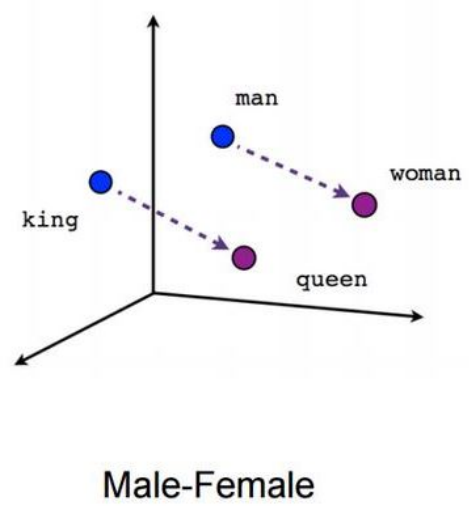
\includegraphics[width=4.5cm]{plots/word2vec.png}%
%       \caption*{https://www.tensorflow.org/tutorials/word2vec/}
%     \end{figure}    
%   \end{minipage}
% \end{vbframe}
%%%%%%%%%%%%%%%%%%%%%%%%%%%%%%%%%%%%%%%%%%%%%%%%%%%%%%%%%%%%%%%%%%
%%%%%%%%%%%%%%%%%%%%%%%%%%%%%%%%%%%%%%%%%%%%%%%%%%%%%%%%%%%%%%%%%%
\begin{vbframe}{Long-Term Dependencies}
  
  \begin{itemize}
    \item Here, $\bm{z}^{[t]} = \sigma(\bm{V}^\top \bm{z}^{[t-1]} + \bm{W}^\top \xv^{[t]} + \bm{b})$
    \item It follows that:
    $$ \frac{d \bm{z}^{[t]}}{d\bm{z}^{[t-1]}} = \text{diag}(\sigma' (\bm{V}^\top \bm{z}^{[t-1]} + \bm{W}^\top \xv^{[t]} + \bm{b})) \bm{V}^\top = \bm{D}^{[t-1]} \bm{V}^\top $$
    $$ \frac{d \bm{z}^{[t-1]}}{d\bm{z}^{[t-2]}} = \text{diag}(\sigma' (\bm{V}^\top \bm{z}^{[t-2]} + \bm{W}^\top \xv^{[t-1]} + \bm{b})) \bm{V}^\top= \bm{D}^{[t-2]} \bm{V}^\top $$
    $$ \vdots $$
    $$ \frac{d \bm{z}^{[2]}}{d\bm{z}^{[1]}} = \text{diag}(\sigma' (\bm{V}^\top \bm{z}^{[1]} + \bm{W}^\top \xv^{[2]} + \bm{b})) \bm{V}^\top = \bm{D}^{[1]} \bm{V}^\top $$
    
    $$ \frac{d L}{d \bm{z}¸^{[1]}} = \frac{d L}{d \bm{z}^{[t]}} \frac{d \bm{z}^{[t]}}{d \bm{z}^{[t-1]}} \dots \frac{d \bm{z}^{[2]}}{d \bm{z}^{[1]}} = \bm{D}^{[t-1]} \bm{D}^{[t-2]}   \text{ . . . } \bm{D}^{[1]} (\bm{V}^\top)^{[t-1]}$$
%    $$ \frac{d \bm{z}^{[1]}}{d\bm{x}^{[1]}} = \text{diag}(\sigma' (\bm{V}^\top \bm{z}^{[0]} + \bm{W}^\top \xv^{[1]} + \bm{b})) \bm{W}^\top$$
    \item Therefore, for an arbitrary time-step $i$ in the past, $\frac{d\bm{z}^{[t]}}{d\bm{z}^{[i]}}$ will contain the term $(\bm{V}^\top)^{t-i}$ within it (this follows from the chain rule).
    \item Based on the largest eigenvalue of $\bm{V}^\top$, the presence of the term $(\bm{V}^\top)^{t-i}$ can either result in vanishing or exploding gradients.
    \item This problem is quite severe for RNNs (as compared to feedforward networks) because the \textbf{same} matrix $\bm{V}^\top$ is multiplied several times. \href{https://tinyurl.com/vangrad}{\beamergotobutton{Click here}}
    \item As the gap between $t$ and $i$ increases, the instability worsens.
    \item It is quite challenging for RNNs to learn long-term dependencies. The gradients either \textbf{vanish} (most of the time) or \textbf{explode} (rarely, but with much damage to the optimization).
    \item That happens simply because we propagate errors over very many stages backwards.
  \end{itemize}
  
  \framebreak
  \begin{itemize}
    \item Recall, that we can counteract exploding gradients by implementing gradient clipping.
    \item Even if we assume that the parameters are such that the recurrent network is stable (can store memories, with gradients not exploding), the difficulty with long-term dependencies arises from the exponentially smaller weights given to long-term interactions (involving the multiplication of many Jacobians) compared to short-term ones.
    \item A more sophisticated solution is needed for the vanishing gradient problem in RNNs.
  \end{itemize}
%\framebreak
%  \begin{itemize}
%    \item The \textbf{vanishing gradient problem} is heavily dependent on the parameter initialization method, but in particular on the choice of the activation functions.
%    \begin{itemize}
%      \item For example, the sigmoid maps a real number into a \enquote{small} range (i.e. $[0, 1]$).
%      \item As a result, large regions of the input space are mapped into a very small range.
%      \item Even a huge change in the input will only produce a small change in the output. Hence, the gradient will be small.
%      \item This becomes even worse when we stack multiple layers of such non-linearities on top of each other (For instance, the first layer maps a large input to a smaller output region, which will be mapped to an even smaller region by the second layer, which will be mapped to an even smaller region by the third layer and so on..).
%      \item We can avoid this problem by using activation functions which do not have the property of \enquote{squashing} the input.
%      \item The most popular choice is obviously the Rectified Linear Unit (ReLU) which maps $x$ to $max(0,x)$.
%      \item The really nice thing about ReLU is that the gradient is either $0$ or $1$, which means it never saturates. Thus, gradients can't vanish.
%      \item The downside of this is that we can obtain a \enquote{dead} ReLU. It will always return $0$  and consequently never learn because the gradient is not passed through.
%    \end{itemize}
%    \item To avoid exploding gradients, we simply clip the norm of the gradient at some threshold $h$ (see chapter 4): $$\text{if  } ||\nabla W|| > \text h: \nabla W \leftarrow \frac{h}{||\nabla W||} \nabla W $$
%  \end{itemize}
\end{vbframe}
%%%%%%%%%%%%%%%%%%%%%%%%%%%%%%%%%%%%%%%%%%%%%%%%%%%%%%%%%%%%%%%%%%
%%%%%%%%%%%%%%%%%%          REFERENCES          %%%%%%%%%%%%%%%%%%
%%%%%%%%%%%%%%%%%%%%%%%%%%%%%%%%%%%%%%%%%%%%%%%%%%%%%%%%%%%%%%%%%%
\begin{vbframe}
\frametitle{References}
\footnotesize{
\begin{thebibliography}{99}
%%%%%%%%%%%%%%%%%%%%%%%%%%%%%%%%%%
\bibitem[Ian Goodfellow et al., 2016]{1} Ian Goodfellow, Yoshua Bengio and Aaron Courville (2016)
\newblock Deep Learning
\newblock \emph{\url{http://www.deeplearningbook.org/}}
%%%%%%%%%%%%%%%%%%%%%%%%%%%%%%%%%%
\bibitem[Andrej Karpathy., 2015]{1} Andrej Karpathy (2015)
\newblock The Unreasonable Effectiveness of Recurrent Neural Networks
\newblock \emph{\url{http://karpathy.github.io/2015/05/21/rnn-effectiveness/}}
%%%%%%%%%%%%%%%%%%%%%%%%%%%%%%%%%%
\end{thebibliography}
}
\end{vbframe}
%%%%%%%%%%%%%%%%%%%%%%%%%%%%%%%%%%%%%%%%%%%%%%%%%%%%%%%%%%%%%%%%%%
%%%%%%%%%%%%%%%%%%%%%%%%%%%%%%%%%%%%%%%%%%%%%%%%%%%%%%%%%%%%%%%%%%

\endlecture
\end{document}
